\chapter{\CoP\,-- A Survey of Important Results}
\label{ch:copsurvey}

This chapter surveys several results that are significant to this
thesis or to \COP in general. These predominantly pertain to
characterizations of \COP, algorithmic tests to check for \COP (COT),
optimization problems on binary matrices that do not have \COP and
some applications of \COP.

\tnote[important]{ADD: have a few lines about organization of chapter}

\tnote{DEFINE COP SOMEWHERE}

\section{\COP in Graph Theory}

\COP is closely connected to several types of graphs by way of
describing certain combinatorial graph properties. There are also
certain graphs, like convex bipartite graphs, that are defined solely
by some of its associated matrix having \COP.  In this section we will
see the relevance of \cop to graphs.  To see this we introduce certain
binary matrices that are used to define graphs in different
ways. While adjacency matrix is perhaps the most commonly used such
matrix, Definition~\ref{def:graphmatrices} defines this and a few
more.

\begin{definition}{\emph{Matrices that define
      graphs.\cite[Def.~2.4]{d08phd}}} %
  \label{def:graphmatrices} %
  Let $G$ and $H$ be defined as follows. $G = (V,E_G)$ is a graph with
  vertex set $V = \{v_i \mid i \in [n]\}$ and edge set $E_G \subseteq
  \{(v_i,v_j) \mid i, j \in [n]\}$ such that $|E_G| = m$. $H = (A, B,
  E_H)$ is a bipartite graph with partitions $A = \{a_i \mid i \in
  [n_a]\}$ and $B = \{b_i \mid i \in [n_b]\}$.
  \begin{enumerate}[{\ref{def:graphmatrices}}--i.]
  \item \emph{Adjacency matrix} of $G$ is the symmetric $n \times n$
    binary matrix $M$ with $m_{i,j} = \un$ \iff $(v_i,v_j) \in E_G$
    for all $i,j \in [n]$.
  \item \emph{Augmented adjacency matrix} of $G$ is obtained from its
    adjacency matrix by setting all main diagonal elements to \un, \ie
    $m_{i,i} = \un$ for all $i \in [n]$.
  \item \emph{Maximal clique matrix} or \emph{vertex-clique incidence
      matrix} of $G$ is the $n \times k$ binary matrix $M$ with
    $m_{i,j} = \un$ \iff $v_i \in C_j$ for all $i \in [n], j \in [k]$
    where $\{C_j \mid j \in [k]\}$ is the set of maximal cliques of
    $G$.
  \item \emph{Half adjacency matrix} of $H$ is the $n_a \times n_b$
    binary matrix $M$ with $m_{i,j} = \un$ \iff $(a_i, b_j) \in E_H$
  \end{enumerate}
\end{definition}
\qed

\begin{figure}[t]
  \centering
  \begin{tabular}[h]{cccl}
    \figtabsize
    ${\bf G_1}$: 
    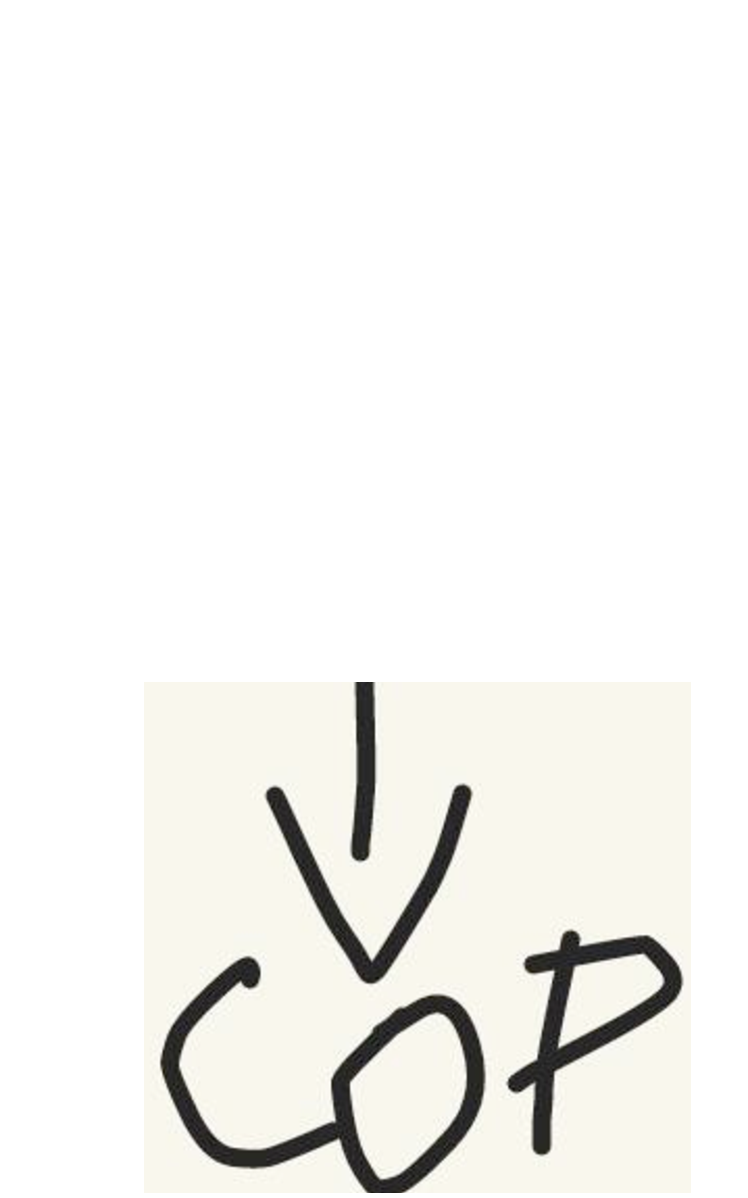
\includegraphics[scale=0.2]{../img/ex1_concaveroundgr.pdf} &
    ${\bf G_2}$: 
    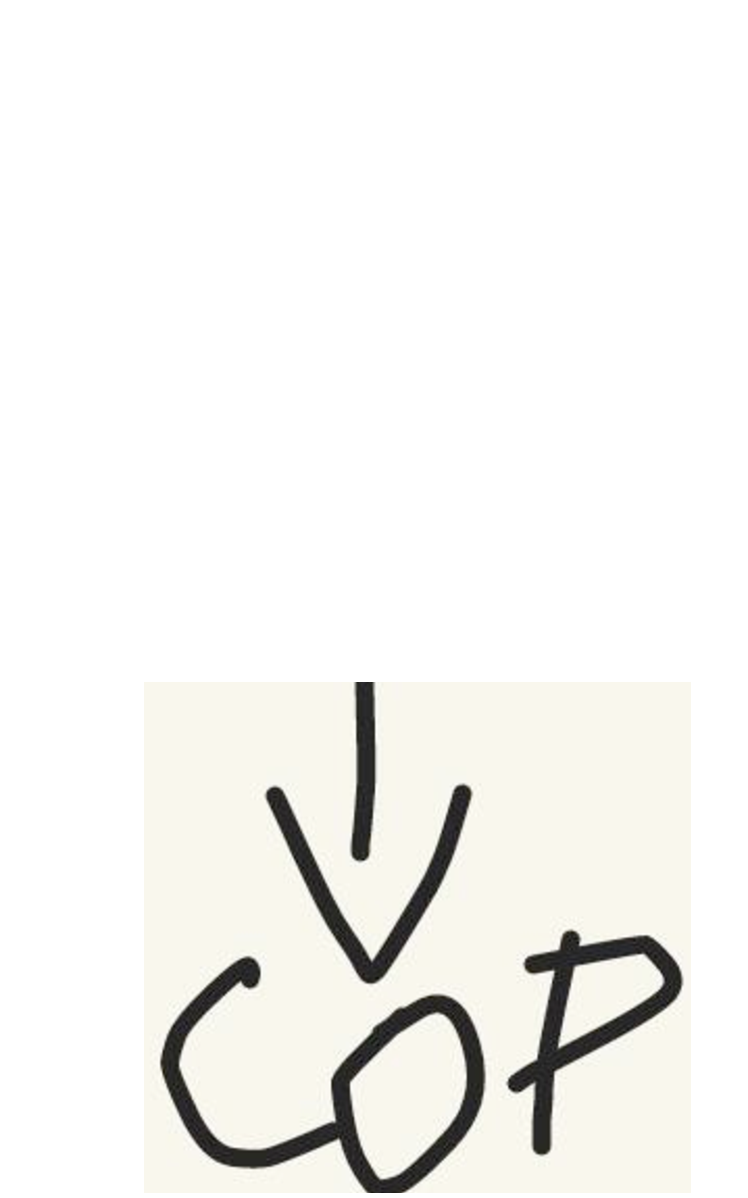
\includegraphics[scale=0.2]{../img/ex2_intervalgr.pdf} &
    ${\bf H}$: 
    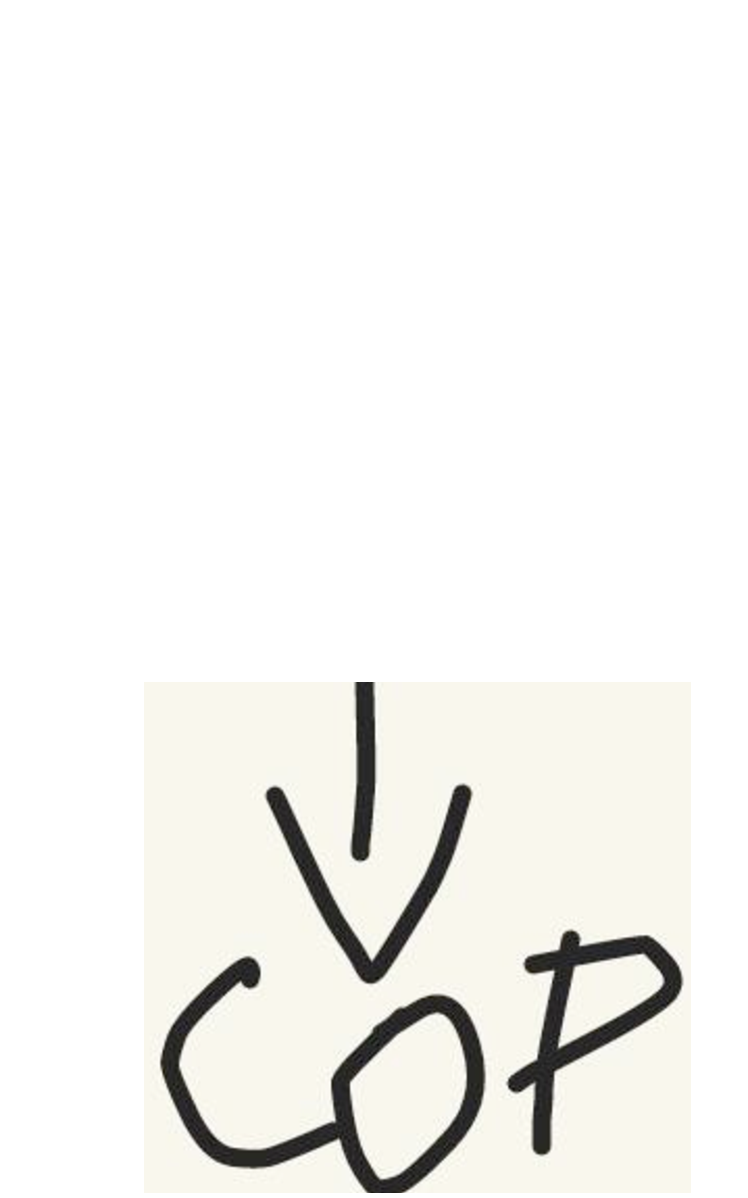
\includegraphics[scale=0.2]{../img/ex2_intervalgr.pdf} &
    \begin{tabular}[h]{l|llll}
      % ${\bf B}$:
      % &&&&\\
      ${\bf C}$ &$w_1$ &$w_2$ &$w_3$ &$w_4$\\
      \hline
      $u_1$ &\un   &\un   &0     &0   \\
      $u_2$ &\un   &\un   &\un   &\un \\
      $u_3$ &0     &0     &\un   &\un \\
      $u_4$ &0     &\un   &\un   &0   \\
      $u_5$ &\un   &\un   &\un   &0   
    \end{tabular}
  \end{tabular}\\

  \begin{tabular}{lll} 
    \begin{tabular}[h]{l|lll lll}
      % ${\bf A_1}$:  
      %&&&&&&\\
      ${\bf A_1}$ &$v_1$ &$v_2$ &$v_3$ &$v_4$ &$v_5$ &$v_6$\\
      \hline
      $v_1$     &0     &\un   &\un  &0     &\un   &\un \\
      $v_2$     &\un   &0     &\un  &\un   &0     &\un \\
      $v_3$     &\un   &\un   &0    &\un   &\un   &0   \\
      $v_4$     &0     &\un   &\un  &0     &0     &0   \\
      $v_5$     &\un   &0     &\un  &0     &0     &0   \\
      $v_6$     &\un   &\un   &0    &0     &0     &0   
    \end{tabular}
    & 
    \begin{tabular}[h]{l|llll}
      % ${\bf B}$:  
      %&&&&\\
      ${\bf B}$&$c_1$ &$c_2$ &$c_3$ &$c_4$\\
      \hline
      $v_1$ &\un   &\un   &\un   &0   \\
      $v_2$ &\un   &0     &0     &0   \\
      $v_3$ &0     &\un   &0     &0   \\
      $v_4$ &0     &0     &\un   &\un \\
      $v_5$ &0     &\un   &\un   &0   \\
      $v_6$ &0     &0     &0     &\un  
    \end{tabular}
    & 
    \\    
    && \\
    \begin{tabular}[h]{l|llllll}
      % ${\bf A_2}$:  
      %&&&&&&\\
      ${\bf A_2}$&$v_1$ &$v_2$ &$v_3$ &$v_4$ &$v_5$ &$v_6$\\
      \hline
      $v_1$ &\un   &\un   &\un  &0     &\un   &\un \\
      $v_2$ &\un   &\un   &\un  &\un   &0     &\un \\
      $v_3$ &\un   &\un   &\un  &\un   &\un   &0   \\
      $v_4$ &0     &\un   &\un  &\un   &0     &0   \\
      $v_5$ &\un   &0     &\un  &0     &\un   &0   \\
      $v_6$ &\un   &\un   &0    &0     &0     &\un 
    \end{tabular}    
    &
    \begin{tabular}[h]{l|llllll}
      % ${\bf A_3}$:  
      %&&&&&&\\
      ${\bf A_2'}$ &$v_1$ &$v_6$ &$v_2$ &$v_4$ &$v_3$ &$v_5$\\
      \hline
      $v_1$ &\un   &\un   &\un  &0     &\un   &\un \\
      $v_6$ &\un   &\un   &\un  &0     &0     &0   \\
      $v_2$ &\un   &\un   &\un  &\un   &\un   &0   \\
      $v_4$ &0     &0     &\un  &\un   &\un   &0   \\
      $v_3$ &\un   &0     &\un  &\un   &\un   &\un \\
      $v_5$ &\un   &0     &0    &0     &\un   &\un 
    \end{tabular}
   & \\


% ex3_convexbipartitegr.png  
  \end{tabular}

  

  \caption[\figtabsize Matrices defined in
  Def.~\ref{def:graphmatrices}]{\figtabsize $A_1$ is the
    {\em adjacency matrix} and $A_2$ is the {\em augmented adjacency matrix} of
    $G_1$. $A_2'$ is obtained from $A_2$ by permuting its rows
    and columns to achieve {\em \CROP order}, \ie $A_2$ has
    \CROP\,-- thus $G_1$
    is {\em a concave-round graph} (Def.~\ref{def:graphwithcop}~\ref{def::concave-round})
    and {\em a circular-arc graph} (Tab.~\ref{tab:graphmatrices})
    $B$ is the maximal clique matrix of $G_2$ and has \COP\,-- thus $G_2$ is an
    {\em interval graph}(Def.~\ref{def:graphwithcop}~\ref{def::concave-round}). $C$ is
    the half adjacency matrix of bipartite graph $H$ and has \COP on
    rows -- thus $H$ is {a convex bipartite graph}.} 
  \label{fig:graphmatrices}
\end{figure}


Now we will see in Definition~\ref{def:graphwithcop} certain graph
classes that is related to \COP or \CROP.\\

{\tt tab~\ref{tab:graphmatrices} -}   \tnote{have an abridged version of table 2.1 in dom}

\begin{table}[htbp]
  \centering
 \caption{\figtabsize **** Graph matrices}
  \label{tab:graphmatrices}
\end{table}

%\hrule
\begin{definition}{\emph{Graphs that relate to
      COP.\cite[Def.~2.5]{d08phd}}} %
   \label{def:graphwithcop} %
   Let $G$ be a graph and $H$ be a bipartite graph.

   \begin{enumerate}[\ref{def:graphwithcop}--i.]
   \item $G$ is \emph{convex-round} if its adjacency matrix has the
     \CROP.
   \item \label{def::concave-round} $G$ is \emph{concave-round} if its augmented adjacency matrix
     has \CROP. \tnote{cite BHY00} \tnote[minor]{add CROP to glossary}
   \item $G$ is an \emph{interval graph} if its vertices can be mapped
     to intervals on the real line \stt two vertices are adjacent \iff
     their corresponding intervals overlap \tnote{cite Ben59, Haj57}.
     $G$ is an interval graph \iff its maximal clique matrix has COP
     due to the result by \cite{gh64} which states that the maximal
     cliques of interval graph $G$ can be linearly ordered \stt for
     all $v \in V(G)$, cliques containing $v$ are consecutive in the
     ordering.
   \item $G$ is a \emph{unit interval graph} if it is an interval
     graph \stt all intervals have the same length.
   \item $G$ is a \emph{proper interval graph} if it is an interval
     graph \stt no interval properly contains another.
   \item $G$ is a \emph{circular-arc graph} if its vertices can be
     mapped to a set of arcs on a circle \stt two vertices are
     adjacent \iff their corresponding arcs overlap.
   \item $H$ is \emph{convex bipartite} if its half adjacency matrix
     has \COP on either rows or columns.
   \item $H$ is \emph{biconvex bipartite} or \emph{doubly
       convex}\cite{yc95} if its half adjacency matrix has \COP on
     both rows and columns.
   \item $H$ is \emph{circular convex} if its half adjacency matrix
     has \CROP.
   \end{enumerate}
\end{definition}
\qed
%\hrule




%%%%%%                                              %%%%%%
% [pressing]{\ \ \ \ \  is the second level of [pressing]%
%%%%%%                                              %%%%%%
\tnote[pressing]{ADD: As it will be described in detail later in this
  document, isomorphism of certain % classes of graphs, namely chordal
  % graphs, have a close relationship with consecutive-ones property
  % and generalizations of it.  This is perhaps because of how closely
  % COP of a matrix relates to properties of graphs derived from
  % matrices as seen inz the following results.
} \tnote[pressing]{\ \ \ \ \ ADD: peo exists iff chordal. lexicographic BFS
  [tag:chordalGraph]} %
\tnote[pressing]{\ \ \ \ \ ADD: A well known result in %perfect graph theory is that
  % the maximal cliques of an interval graph $G$ can be linearly
  % ordered such that for all $v \in V(G)$, cliques containing $v$ are
  % consecutive in the ordering cite~{gh64}. This clearly means that a
  % graph $G$ is an interval graph if and only if
}%
\tnote[pressing]{\ \ \ \ \ verify from paper the statement of claim.}%
\tnote[pressing]{maximal clique vertex incidence matrix
  of% $G$ has COP.  Also, maximal cliques of any
  % chordal graph can be enumerated in polytime $O(m+n)$
} \tnote[pressing]{\ \ \ \ \ citation?!!}%
\tnote[pressing]{cite~{fg65} uses these results to give the first polynomial
  time algorithm for COT.}%
\tnote[pressing]{\ \ \ \ \ check. how do they use it?}%
\tnote[pressing]{ A bipartite graph is
  convex% (on $R$) if and only if its half adjacency matrix has COP
  % on rows.  The results in cite~{bl76} on COT are based on the
  % result that interval graphs are AT-free chordal graphs.
}%
\tnote[pressing]{\ \ \ \ \ the latter being Tucker's?}%
\tnote[pressing]{\ \ \ \ \ (2) TBD survey
  -- % see blue notes (in notebook) under Graph Isomorphism. namely
  % citations in cite:aas93 (3) a brief on heirarchy of chordal
  % graphs, path graphs, interval graphs, peo, clique tree etc. and
  % results. (4) interval graphs are incomparability graphs. see
  % Golumbic. [tag:classification] (5) finding min length hole in
  % bipartite graph is polynomial time [Sec 3.3.2 in cite:d08phd] (6)
  % theorem 2.2 in cite:d08phd - $G$ is union of v.d. caterpillars iff
  % $M$ has COP in rows. $M$ is edge vertex incidence matrix $(*,2)$
  % of $G$
}%



\section{Matrices with COP}
\label{sec:surveycoptest}
\tnote{Expand on ref:sec:copmatrices}

Figure~\ref{fig:cop-matrix} shows examples of consecutive-ones
property. \tnote[important]{move to general def section? if so, decide
how to cross ref with repetition for completeness of chapter.}

\begin{figure}[t] %[htbp]
  \centering

  {\figtabsize
    \begin{tabular}[h]{l|lcccl}
      $M_1$: & $M_1'$: &&&& $M_2$:\\
      &&&&&\\
      \begin{tabular}[h]{llll}
        $c_1$ & $c_2$ &$c_3$ &$c_4$\\
        &&&\\
        \un & 0   & \un & 0\\
        0   & \un & 0   & \un \\
        \un & 0   & 0   & \un
      \end{tabular}
      &
      \begin{tabular}[h]{llll}
        $c_3$ &$c_1$ &$c_4$& $c_2$\\
        &&&\\
        \un & \un & 0 & 0\\
        0 & 0 & \un & \un \\
        0 & \un & \un & 0
      \end{tabular}
      &&&&
      \begin{tabular}[h]{llll}
        $d_1$ & $d_2$ &$d_3$ &$d_4$\\
        % &&&\\
        &&&\\
        \un & \un & 0 & 0\\
        0 & \un & \un & 0 \\
        0 & \un & 0 & \un 
      \end{tabular}
    \end{tabular}
  }

  \caption[\figtabsize Matrices with and without COP.]{\figtabsize
    Matrices with and without COP. $M_1$ has COP because by permuting
    its columns, $c_1$-$c_4$, one can obtain $M_1'$ where the {\un}s
    in each row are consecutive. $M_2$, however, does not have COP
    since no permutation of its columns, $d_1$-$d_4$, will arrange
    {\un}s in each row consecutively \cite{d08phd}.}

  \label{fig:cop-matrix}
\end{figure}



\section{Optimization problems in COP}
\label{sec:surveycopopt}
\tnote{Expand on ref:sec:optcop}


\section{********* COP in Relational Database Model}
\label{sec:surveyrdbm}
\tnote{Expand on sec:apprdbm} \tnote{(set systems theme)}

\section{********* COP in Graph Isomorphism}
\label{sec:surveygraphiso}
\tnote{Expand on sec:appgraphiso} \tnote{(canonization theme)}

\section{********* Certifying Algorithms}
\label{sec:surveycertalgo}
\tnote{Expand on sec:appcertalgo} \tnote{ (certification McC04 theme)}


\section*{-- REFERENCE CONTENT --}
%%%%%%%%%%%%% listing package for pretty formatting BEGIN
% \lstloadlanguages{C}
% \lstset{language=C, commentstyle=\scriptsize,
%   numberstyle=\tiny, numbers=left,               % Line numbers
%   stepnumber=2,numbersep=5pt,firstnumber=10, 
%   showstringspaces=false,                    % No explicit spaces
%   emph={printf},emphstyle=\underbar,      % Specific formatting
%   emph=[2]{sum},emphstyle=[2]\color{blue},      % Sp format (multiple)
%   emph=[3]{i},emphstyle=[3]\color{red}      % Sp format (multiple)
%   } 

%   \begin{singlespacing}
%     % Text inside "lstlisting" env is verbatim.
%     \begin{lstlisting}[keywordstyle=\textbf]      
% int sum;
% int i; /* for loop variable */ 
% sum = 0; 
% for (i=0, i<n; i++) { 
%   sum += a[i]; 
% } 
% printf{"This is stupid."}
%     \end{lstlisting}
%   \end{singlespacing}

%%%%%%%%%%%%% listing package for pretty formatting END

{%\fontfamily{cmvtt}\selectfont
\color{blue}
\subsection{Matrices with COP}
\label{sec:copmatrices}
As seen earlier, the interval assignment problem (illustrated as the
course scheduling problem in Section~\ref{sec:problem}), is a special
case of the problem we address in this thesis, namely the tree path
labeling problem (illustrated as the \illustrationproblem). The
interval assignment problem and COP problem are equivalent
problems. In this section we will see some of the results that exists
in the literature today towards solving the COP problem and
optimization problems surrounding it.

Recall that a matrix with COP is one whose rows (columns) can be
rearranged so that the {\un}s in every column (row) are in consecutive
rows (columns). COP in binary matrices has several practical applications
in diverse fields including scheduling \cite{hl06}, information
retrieval \cite{k77} and computational biology \cite{abh98}.  Further,
it is a tool in graph theory \cite{mcg04} for interval graph
recognition, characterization of Hamiltonian graphs, planarity testing
\cite{bl76} and in integer linear programming \cite{ht02,hl06}.


The obvious first questions after being introduced to the consecutive
ones property of binary matrices are if COP can be detected
efficiently in a binary matrix and if so, can the COP permutation of
the matrix also be computed efficiently?  Recognition of COP in a
binary matrix is polynomial time solvable and the first such algorithm
was given by \cite{fg65}.  A landmark result came a few years later
when \cite{at72} discovered the families of forbidden submatrices that
prevent a matrix from having COP and most, if not all, results that
came later were based on this discovery which connected COP in binary
matrices to convex bipartite graphs. In fact, the forbidden
submatrices came as a corollary to the discovery that convex bipartite
graphs are AT-free in \cite{at72}\tnote{check}. The first linear
time algorithm for COP testing (COT) was invented by \cite{bl76} using
a data structure called PQ trees.  Since then several COT algorithms
have been invented -- some of which involved variations of PQ trees
\cite{mm96,wlh01,mcc04}, some involved set theory and ICPIA
\cite{wlh02,nsnrs09}, parallel COT algorithms\cite{as95,bs03,ly91} and
certifying algorithms\cite{mcc04}.

The construction of PQ trees in \cite{bl76} draws on the close
relationship of matrices with COP to interval graphs. A PQ tree of a
matrix is one that stores all row (column) permutations of the matrix
that give the COP orders (there could be multiple orders of rows or
columns) of the matrix. This is constructed using an elaborate linear
time procedure and is also a test for planarity\tnote{check check
  check. both interval graph and planarity in this paper?}.  PQR trees
is a generalized data structure based on PQ trees \cite{mm96,mpt98}.
\cite{tm05} describes an improved algorithm to build PQR
trees. \tnote{improv in terms of what?}\cite{wlh02} describes the
simpler algorithm for COT. Hsu also invented PC trees
\cite{wlh01}\tnote{This result first appeared inproc ISAAC92}
which is claimed to be much easier to implement. \cite{nsnrs09}
describes a characterization of consecutive-ones property solely based
on the cardinality properties of the set representations of the
columns (rows); every column (row) is equivalent to a set that has the
row (column) indices of the rows (columns) that have one entries in
this column (row). This is interesting and relevant, especially to
this thesis because it simplifies COT to a great degree. \tnote{it
  reduces the solution search space. fill in the blanks.}

\cite{mcc04} describes a different approach to COT. While all previous
COT algorithms gave the COP order if the matrix has the property but
exited stating negative if otherwise, this algorithm gives an evidence
by way of a certificate of matrix even when it has no COP. This
enables a user to verify the algorithm's result even when the answer
is negative. This is significant from an implementation perspective
because automated program verification is hard and manual verification
is more viable. Hence having a certificate reinforces an
implementation's credibility. Note that when the matrix {\em has} COP,
the COP order is the certificate.  The internal machinery of this
algorithm is related to the weighted betweenness problem
addressed\tnote{in what way??} in \cite{co98}.  \tnote{expand
  on the COP order graph creation and it having to be bipartite for M
  to have COP. and thus an odd cycle being an evidence of no COP.}
\tnote{ where should this go?: (1) cite|jlm97 (application of PQ
  trees in graphics). (2) helly's theorem citation
  19XXdgk-Hellystheorem-Danzer-Gruenbaum-Klee}


\subsection{Optimization problems in COP}
\label{sec:optcop}

So far we have been concerned about matrices that have the consecutive
ones property. However in real life applications, it is rare that data
sets represented by binary matrices have COP, primarily due to the
noisy nature of data available. At the same time, COP is not arbitrary
and is a desirable property in practical data representation
\cite{co98,jkckv04,k77}. In this context, there are several
interesting problems when a matrix does not have COP but is ``close''
to having COP or is allowed to be altered to have COP. These are the
optimization problems related to a matrix which does not have
COP. Some of the significant problems are surveyed in this section.

\tnote{ -- sect 4.1 in cite:d08phd has many results
  surveyed. hardness results, approx. results. results are usually for
  a class of matrices $(a,b)$ where number {\un}s in columns and rows
  are restriced to $a$ and $b$ . -- problem of flipping at most $k$
  entries of $M$ to make it attain COP. this is NP complete
  cite:b75-phd}\tnote{(1) scite:lb62 showed that interval graphs
  are AT-free.  describe AT (2) show the close relationship b/w COP
  and graphs sec 2.2, pg 31} \cite{at72} showed that a matrix that
does not have COP have certain substructures that prevent it from
having COP. Tucker classified these forbidden substructures into five
classes of submatrices. This result is presented in the context of
convex bipartite graphs which \cite{at72} proved to be
AT-free\tnote{ check this up. give details. - doms'}. By
definition, convex bipartite graph have half adjacency matrices that
have COP on either rows or columns (graph is biconvex if it has COP on
both)\cite{d08phd}. A half adjacency matrix is a binary matrix
representing a bipartite graph as follows. The set of rows and the set
of columns form the two partitions of the graph. Each row node is
adjacent to those nodes that represent the columns that have {\un}s in
the corresponding row. \cite{at72} proves that this bipartite graph
has no asteroidal triple if and only if the matrix has COP and goes on
to identify the forbidden substructures for these bipartite
graphs. The matrices corresponding to these substructures are the
forbidden submatrices.

Once a matrix has been detected to not have COP (using any of the COT
algorithms mentioned earlier), it is naturally of interest to find out
the smallest forbidden substructure (in terms of number of rows and/or
columns and/or number of entries that are {\un}s). \cite{d08phd}
discusses a couple of algorithms which are efficient if the number of
{\un}s in a row is small. This is of significance in the case of
sparse matrices where this number is much lesser than the number of
columns. $(*,\Delta)${\em -matrices} are matrices with no restriction
on number of {\un}s in any column but has at most $\Delta$ {\un}s in
any row. {\sc Min COS-R (Min COS-C), Max COS-R (Max COS-C)} are
similar problems which deals with inducing COP on a matrix. In {\sc
  Min COS-R (Min COS-C)} the question is to find the minimum number of
rows (columns) that must be deleted to result in a matrix with COP.
In the dual problem {\sc Max COS-R (Max COS-C)} the search is for the
maximum number of rows (columns) that induces a submatrix with
COP. Given a matrix $M$ with no COP, \cite{b75-phd} shows that finding
a submatrix $M'$ with all columns\tnote{check if b75 deals with
  COP col or COP row. also is it any submatrix with k less than r rows
  or submatrix must have all columns?} but a maximum cardinality
subset of rows such that $M'$ has COP is NP complete. \cite{hg02}
corrects an error of the abridged proof of this reduction as given in
\cite{gj79}.  \cite{d08phd} discusses all these problems in detail
giving an extensive survey of the previously existing results which
are almost exhaustively all approximation results and hardness
results. Taking this further, \cite{d08phd} presents new results in
the area of parameterized algorithms for this
problem\tnote{elaborate - what are the results?}.

Another problem is to find the minimum number of entries in the matrix
that can be toggled to result in a matrix with COP.  \cite{v85}
discusses approximation of {\sc COP Augmentation} which is the problem
of changing of the minimum number of zero entries to {\un}s so that
the resulting matrix has COP. As mentioned earlier, this problem is
known to be NP complete due to \cite{b75-phd}. \cite{v85} also proves,
using a reduction to the longest path problem, \tnote{or is it a
  survey of another result?  check.} that finding a Tucker's forbidden
submatrix of at least $k$ rows is NP complete. \tnote{how is this
  different from booth's 75 result??}  \tnote{where should this go?
  cite|tz04 (approx submatrix with COP sparse matrices)}

\cite{jkckv04} discusses the use of matrices with almost-COP (instead
of one block of consecutive {\un}s, they have $x$ blocks, or {\em
  runs}, of consecutive {\un}s and $x$ is not too large) in the
storage of very large databases.  The problem is that of reordering of
a binary matrix such that the resulting matrix has at most $k$ runs of
{\un}s. This is proved to be NP hard using a reduction from the
Hamiltonian path problem.\tnote{Theorem 2.1 in jkckv} \tnote{(1) A
  connection of COP problem to the travelling salesman problem is also
  introduced. what does this mean? -- COP can be used as a tool to
  reorder $0.5T \le runs(M) \le T$. (2) The optimization version of
  the $k$-run problem, i.e. minimization of number of blocks of ones
  is proven to be NP complete by cite:k77}\tnote{are these two the
  same?} \tnote{what is the reduction?} \tnote{other problems similar
  to COP -- cite:ckl96 (ILP, circ ones, one drop) -- cite:th98
  (generalization of COP - minimax, biotonic column) Tucker} }
















\theendnotes\tnote{remove if none.} 